%============================================================================
% tento soubor pouzijte jako zaklad
% (c) 2008 Michal Bidlo
% E-mail: bidlom AT fit vutbr cz
%============================================================================
% kodovaní: iso-8859-2 (zmena prikazem iconv, recode nebo cstocs)
%----------------------------------------------------------------------------
% zpracování: make, make pdf, make desky, make clean
% připomínky posílejte na e-mail: bidlom AT fit.vutbr.cz
% vim: set syntax=tex encoding=latin2:
%============================================================================
\documentclass[cover]{fitthesis} % odevzdani do wisu - odkazy, na ktere se da klikat
%\documentclass[cover,print]{fitthesis} % pro tisk - na odkazy se neda klikat
%\documentclass[english,print]{fitthesis} % pro tisk - na odkazy se neda klikat
%      \documentclass[english]{fitthesis}
% * Je-li prace psana v anglickem jazyce, je zapotrebi u tridy pouzit 
%   parametr english nasledovne:
%      \documentclass[english]{fitthesis}
% * Neprejete-li si vysazet na prvni strane dokumentu desky, zruste 
%   parametr cover

% zde zvolime kodovani, ve kterem je napsan text prace
% "latin2" pro iso8859-2 nebo "cp1250" pro windows-1250, "utf8" pro "utf-8"
%\usepackage{ucs}
\usepackage[utf8]{inputenc}
\usepackage[T1, IL2]{fontenc}
\usepackage{url}
\usepackage{graphicx}
\usepackage{gensymb}
\DeclareUrlCommand\url{\def\UrlLeft{<}\def\UrlRight{>} \urlstyle{tt}}

%zde muzeme vlozit vlastni balicky


% =======================================================================
% balíček "hyperref" vytváří klikací odkazy v pdf, pokud tedy použijeme pdflatex
% problém je, že balíček hyperref musí být uveden jako poslední, takže nemůže
% být v šabloně
\ifWis
\ifx\pdfoutput\undefined % nejedeme pod pdflatexem
\else
  \usepackage{color}
%  \usepackage[unicode,colorlinks,hyperindex,plainpages=false,pdftex]{hyperref}
  \usepackage[unicode,colorlinks,hyperindex,plainpages=false]{hyperref}
  \definecolor{links}{rgb}{0.4,0.5,0}
  \definecolor{anchors}{rgb}{1,0,0}
  \def\AnchorColor{anchors}
  \def\LinkColor{links}
  \def\pdfBorderAttrs{/Border [0 0 0] }  % bez okrajů kolem odkazů
  \pdfcompresslevel=9
\fi
\fi

%Informace o praci/projektu
%---------------------------------------------------------------------------
\projectinfo{
  %Prace
  project=SP,            %typ prace BP/SP/DP/DR
  year=2013,             %rok
  date=\today,           %datum odevzdani
  %Nazev prace
  title.cs={Pokročilý simulátor mikrokontrolerů rodiny MSP430},  %nazev prace v cestine
  title.en={Advanced Simulator of MSP430 Microcontrollers}, %nazev prace v anglictine
  %Autor
  author={Jan Kaluža},   %jmeno prijmeni autora
  author.title.p=Bc., %titul pred jmenem (nepovinne)
  %author.title.a=PhD, %titul za jmenem (nepovinne)
  %Ustav
  department=MSK, % doplnte prislusnou zkratku: UPSY/UIFS/UITS/UPGM
  %Skolitel
  supervisor={Zdeněk Vašíček}, %jmeno prijmeni skolitele
  supervisor.title.p=Ing.,   %titul pred jmenem (nepovinne)
  supervisor.title.a={Ph.D.},    %titul za jmenem (nepovinne)
  %Klicova slova, abstrakty, prohlaseni a podekovani je mozne definovat 
  %bud pomoci nasledujicich parametru nebo pomoci vyhrazenych maker (viz dale)
  %===========================================================================
  %Klicova slova
  keywords.cs={MSP430, simulace, DEVS, Python, Qt, C++}, %klicova slova v ceskem jazyce
  keywords.en={MSP430, simulation, DEVS, Python, Qt, C++}, %klicova slova v anglickem jazyce
  %Abstract
%% YARDA: Návrh abstraktu.
  abstract.cs={
}, % abstrakt v ceskem jazyce
%% YARDA: Český návrh není přeložen.
abstract.en={}, % abstrakt v anglickem jazyce
  %Prohlaseni
  declaration={Prohlašuji, že jsem tuto bakalářskou práci vypracoval samostatně pod vedením pana Ing. Zdeňka Vašíčka, Ph.D.},
  %Podekovani (nepovinne)
%   acknowledgment={Zde je možné uvést poděkování vedoucímu práce a těm, kteří poskytli odbornou pomoc.} % nepovinne
}

%Abstrakt (cesky, anglicky)
%\abstract[cs]{Do tohoto odstavce bude zapsán výtah (abstrakt) práce v českém jazyce.}
%\abstract[en]{Do tohoto odstavce bude zapsán výtah (abstrakt) práce v anglickém jazyce.}

%Klicova slova (cesky, anglicky)
%\keywords[cs]{Sem budou zapsána jednotlivá klíčová slova v českém jazyce, oddělená čárkami.}
%\keywords[en]{Sem budou zapsána jednotlivá klíčová slova v anglickém jazyce, oddělená čárkami.}

%Prohlaseni
%\declaration{Prohlašuji, že jsem tuto bakalářskou práci vypracoval samostatně pod vedením pana X...
%Další informace mi poskytli...
%Uvedl jsem všechny literární prameny a publikace, ze kterých jsem čerpal.}

%Podekovani (nepovinne)
%\acknowledgment{V této sekci je možno uvést poděkování vedoucímu práce a těm, kteří poskytli odbornou pomoc
%(externí zadavatel, konzultant, apod.).}

\begin{document}
  % Vysazeni titulnich stran
  % ----------------------------------------------
  \maketitle
  % Obsah
  % ----------------------------------------------
  \tableofcontents
  
  % Seznam obrazku a tabulek (pokud prace obsahuje velke mnozstvi obrazku, tak se to hodi)
  % \listoffigures
  % \listoftables 

  % Text prace
  % ----------------------------------------------
  % 
% Pekny den,
% 
% konecne jsem se dostal k precteni textu. Mam v soucasne dobe nasledujici
% poznamky:
% DONE 1) od druheho odstavce kap. 3 bych z toho udelal podkapitolu "UVOD"
% DONE 2) po uvodu bych dal schema blokove a soucasny 4. odstavec trosku rozvedl
% DONE 3) lepe formulovat vsechny instrukce jsou => Instrukce jsou kodovany
% pomoci 16, 32 nebo 48 bitu pricemz operacni kod je situovan vzdy v
% prvnich 16 bitech.
% DONE 4) kap 3 lepe clenit - periferie dat do podkapitoly napr. Zakladni
% periferie; at je z obsahu zrejme, ze se zabyvate IS, periferiemi, apod
% DONE 5) kap 4  by  bylo vhodne prejmenovat, aby bylo zrejme, ze budete
% popisovat obecne platnou zalezitost; nicmene pokud by mel rozsah zustat
% spise maly, lepsi by bylo text pridat do kapitoly zabyvajici se
% navrhem/implementaci ci jinam
% DONE 6) kap 5 - vystizneji nazvat - napr. "Navrh udalostne rizeneho simulatoru"
% DONE 7) Cílem této kapitoly je návrh simulátoru => Cílem této kapitoly je
% popsat strukturu navrzeneho simulatoru
% DONE 8) Pred kapitolu 5 bych dal kapitolu "Udalostne rizena simulace" a do ni
% rozebral a) co to je a b) existujici systemy vcetne DEVS; v kapitole 5
% se jen odkazat,ze to bude vyuzito
% DONE 9) v ramci kap 5 bych asi nazyval komponentu msp430 simulacnim jadrem,
% ale to je spise k diskusi
% DONE 10) kap 5 by mela zacit "Struktura navrzeneho simulatoru", kde by se
% zminilo jadro + rozsireni (podpora pro periferie) + nad tim GUI; teprve
% pote se zabyvat popisem jednotlivych casti
% DONE 11) zatim bych text v kap5 nechal byt a jakmile si budete myslet, ze je
% kompletni, detailne bych jej procetl a napsal pripominky; nyni se mi
% zda, ze tam je spoustu informaci, ale chtelo by je to trosku utribit
%       chtelo by to napsat zminku, ktere mechanismy se budou z DEVS
% pouzivat (nikoliv vsak uplne detaily - ty budou az v implementaci) -
% napr. "Komponenty budou ke komunikaci vyuzivat ...."

\chapter{Úvod}

Mikrokontrolery (MCU) jsou monolitické integrované obvody obsahující mikroprocesor, paměť pro uložení programu, paměť pro jeho běh a další periferie
rozšiřující jeho funkčnost. Vyznačují se jednoduchostí, kompaktností a malou spotřebou. Používají se tak proto především pro jednoúčelová zařízení a 
vestavěné (embedded) systémy.

Při návrhu vestavěných systémů je v praxi často používána simulace. Díky využití simulátoru daného mikrokontroleru (případně celého vestavěného systému) lze ověřit funkčnost systému již při jeho návrhu aniž by bylo nutné vynaložit náklady na prvotní prototypy. Simulační čas lze zrychlit nebo naopak zpomalit a tím jednodušeji prozkoumat vybrané jevy. Simulace může rovněž zjednodušit hledání problémů viděných na reálném hardwaru, kdy jejich příčiny nelze prostým zkoumáním reálného systému jednoduše odhalit. Při použití simulace je také jednodušší vyzkoušet případné změny systému a zkoumat nové postupy bez dalšího zvýšení nákladů. Nejen z těchto důvodů je tedy simulace vestavěných systémů užitečná a má smysl se jí zabývat.

Tato semestrální práce si dává za cíl návrh jednoduše rozšiřitelného pokročilého simulátoru mikrokontrolerů rodiny MSP430 od výrobce Texas Instruments. Tyto mikrokontrolery jsou hojně rozšířené především díky své nízké ceně, malé spotřebě a jednoduchosti práce s nimi. Lze je nalézt například i v platformě FITkit používané k výukovým účelům Fakultou informačních technologií Vysokého učení technického v Brně. Simulátor navrhovaný v této práci je navrhován právě jako doplňující prostředek pro vývoj aplikací pro tuto platformu, avšak bude moci být použit i samostatně. V současné době není obdobný software pod svobodnou licencí dostupný.

Tento semestrální projekt je rozdělen do pěti kapitol.

První kapitola obsahuje úvod. Dále následuje kapitola stručně popisující strukturu mikrokontroleru MSP430, jeho instrukční sadu, základní interní periferie a formáty používané pro uložení binárního kódu tohoto mikrokontroleru. Třetí kapitola se zabývá událostně řízenou simulací, konkrétně pak formalismem DEVS. Ve čtvrté kapitole je proveden samotný návrh simulátoru. Na závěr je navržený simulátor zhodnocen.

% Mikrokontroler MSP430, kterého se táto práce týká, je postaven na von Neumannově architektuře (má tedy společnou paměť pro data i program). Paměť je adresována po bytech složených z 8 bitů a páry bytů tvoří 16bitové little-endian slova.


\chapter{Mikrokontroler MSP430}

Tato kapitola stručně shrnuje základy architektury mikrokontrolerů rodiny MSP430. Nesnaží se však kompletně nahradit jejich dokumentaci \cite{msp430family} \cite{msp430book}, ačkoliv z ní vychází. Pro návrh a implementaci kompletního simulátoru nejsou informace v této kapitole dostačující, ale byly vybrány s ohledem na úvod do problematiky mikrokontrolerů MSP430 a pochopení následujících kapitol a činnosti navrhovaného simulátoru.

\begin{figure}[ht]
\centering
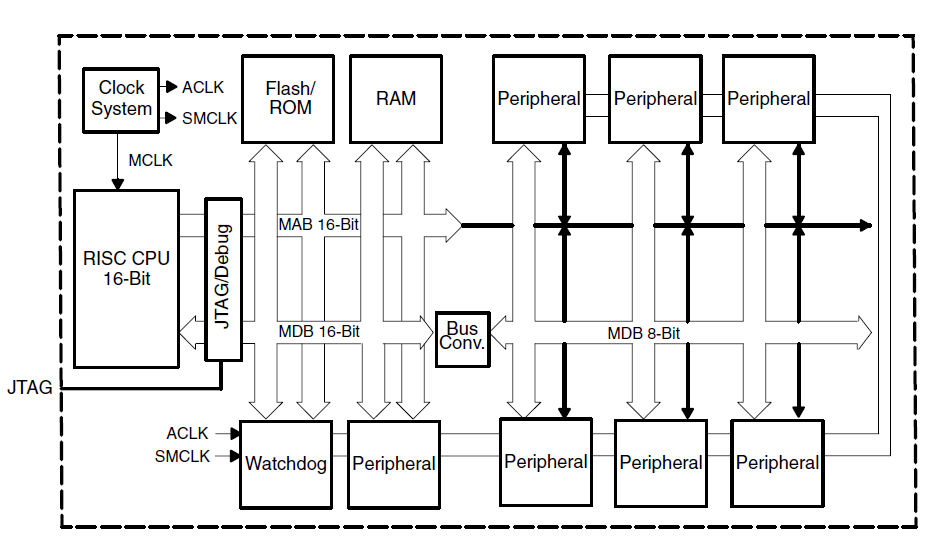
\includegraphics[trim=0cm 0cm 0cm 0cm, scale=0.5]{fig/msp430block}
\caption{Blokové schéma mikrokontroleru MSP430.}
\label{fig:msp430block}
\end{figure}

Mikrokontroler je rozdělen na několik bloků, které lze vidět na obrázku \ref{fig:msp430block}. Jádrem celého mikrokontroleru je 16bitový mikroprocesor
vykonávající instrukce programu definované jeho instrukční sadou. Frekvence mikroprocesoru a všech dalších periferií je řízena systémem hodin (Clock System). K mikroprocesoru je pomocí 16bitové adresové sběrnice a 16bitové datové sběrnice připojena paměť programu (Flash/ROM) a paměť dat (RAM). Další doplňující periferie jsou pak adresovány adresovou sběrnicí o menší šířce v závislosti na modelu mikrokontroleru. Datová sběrnice periferií je buď 16bitová nebo 8bitová v závislosti na potřebě konkrétní periferie.

Jednotlivé bloky mikrokontroleru MSP430 jsou podrobněji popsány dále v této kapitole.

\section{Mikroprocesor a instrukční sada}

Mikrokontrolery rodiny MSP430 obsahují 16bitový mikroprocesor (CPU) a 16 registrů, každý o kapacitě 16 bitů. První čtyři registry mají speciální účel. Registr R0 slouží jako ukazatel na aktuální instrukci (PC - program counter). Register R1 ukazuje na vrchol zásobníku (SP - stack pointer). Register R2 je stavovým registrem (SR - status register) obsahujícím informace o stavu mikroprocesoru. Register R3 je použit pro generování často používaných konstant, takže je není potřeba načítat z paměti. Ostatní registry je možné volně využít v uživatelském programu.

Nejdůležitějšími stavovými bity ve stavovém registru jsou bity N (nastaven pokud je výsledek operace negativní), Z (nastaven pokud je výsledek operace nulový), C (nastaven pokud došlo k přenosu nejvyššího bitu) a V (nastaven pokud došlo při operaci k přetečení).

\subsection{Instrukční sada}

Instrukční sada obsahuje 27 instrukcí. Instrukce jsou kódovány pomocí 16, 32 nebo 48 bitů přičemž operační kód je situován vždy v prvních 16 bitech.

Většina instrukcí pracujících s daty umí pracovat jak s operandem velikosti jednoho bytu, tak s celým slovem. Instrukce lze rozdělit do 3 typů, které se liší i rozdílným kódováním v prvních 16 bitech instrukce uložené v paměti:

\subsubsection{Instrukce s jedním operandem}

V závislosti na operačním kódu (opcode) rozlišuje mikroprocesor následující jednooperandové instrukce (.B značí bytovou formu instrukce):

\begin{itemize}
\item \textbf{RRC(.B)} - 9 bitová rotace s přenosem nejvyššího bitu.
\item \textbf{SWPB} - Záměna horních a spodních 8 bitů v rámci jednoho registru.
\item \textbf{RRA(.B)} - 8 bitový aritmetický posun doprava.
\item \textbf{SXT} - Rozšíření znaménka z 8 bitů na 16 bitů.
\item \textbf{PUSH(.B)} - Uložení operandu na zásobník. Sníží hodnotu SP o 2.
\item \textbf{CALL} - Volání podprogramu. Získá operand, uloží PC na zásobník a do PC uloží hodnotu operandu.
\item \textbf{RETI} - Návrat z přerušení. Obnoví ze zásobníku SP a PC.
\end{itemize}

\subsubsection{Instrukce s dvěma operandy}

Mikrokontroler MSP430 rozlišuje tyto instrukce se dvěma operandy a provádí s nimi následující operace:

\begin{itemize}
\item \textbf{MOV src,dest} - dest = src
\item \textbf{ADD src,dest} - dest += src
\item \textbf{ADDC src,dest} - dest += src + C
\item \textbf{SUBC src,dest} - dest += ~src + C
\item \textbf{SUB src,dest} - dest -= src
\item \textbf{CMP src,dest} - dest - src (Mění pouze stavový registr)
\item \textbf{DADD src,dest} - dest += src + C, BCD.
\item \textbf{BIT src,dest} - dest \& src (Mění pouze stavový registr)
\item \textbf{BIC src,dest} - dest \&= ~src
\item \textbf{BIS src,dest} - dest |= src
\item \textbf{XOR src,dest} - dest \^ = src
\item \textbf{AND src,dest} - dest \&=- src
\end{itemize}

\subsubsection{Podmíněné instrukce}

Podmíněné instrukce jsou typicky instrukce skoků, které provedou skok pouze při splnění určité podmínky (hodnoty konkrétního bitu ze stavového registru). Zpravidla je před nimi volání instrukce CMP pro porovnání dvou hodnot a nastavení stavového registru. Opět je rozlišeno několik druhů podmíněných instrukcí:

\begin{itemize}
\item \textbf{JNE/JNZ} - Provede skok pokud Z==0 (po zavolání CMP se 2 hodnoty nerovnají).
\item \textbf{JEQ/Z} - Provede skok pokud Z==1 (po zavolání CMP se 2 hodnoty rovnají).
\item \textbf{JNC/JLO} - Provede skok pokud C==0 (po zavolání CMP je první neznaménková hodnota menší než druhá).
\item \textbf{JC/JHS} - Provede skok pokud C==1 (po zavolání CMP je první neznaménková hodnota vetší nebo rovna druhé).
\item \textbf{JN} - Provede skok pokud N==1.
\item \textbf{JGE} - Provede skok pokud N==V (po zavolání CMP je první znaménková hodnota vetší nebo rovna druhé).
\item \textbf{JL} - Provede skok pokud N!=V (po zavolání CMP je první znaménková hodnota menší než druhá).
\item \textbf{JMP} - Provede skok vždy.
\end{itemize}

\subsubsection{Časování instrukcí}

Každá instrukce potřebuje ke svému vykonání určitý počet hodinových cyklů. Zpravidla je zapotřebí 1 cyklus pro každý přístup do paměti. Z tohoto pravidla však existuje několik výjimek popsaných v dokumentaci k mikrokontrolerům MSP430.
 
\subsection{Adresové módy}

Mikrokontroler MSP430 pracuje se 7 adresovými módy pro zdrojový operand a 4 adresovými módy (první 4 módy následujícího seznamu) pro operand cílový:

\begin{itemize}
\item \textbf{Registrový mód} - Rn - Operand je uložen v registru Rn.
\item \textbf{Indexový mód} - X(Rn) - Operand je uložen v paměti na adrese Rn + X. X je uloženo v následujícím slově za instrukcí.
\item \textbf{Symbolický mód} - ADDR - Operand je uložen v paměti na adrese PC + X. X je uloženo v následujícím slově za instrukcí.
\item \textbf{Absolutní mód} - \&ADDR - Adresa operandu je uložena v následujícím slově za instrukcí.
\item \textbf{Nepřímý registrový mód} - @Rn - Register Rn ukažuje na umístění operandu.
\item \textbf{Nepřímý mód s automatickou inkrementací} - Register Rn ukazuje na umístění operandu. Rn je inkrementován o hodnotu 1 (přístup k bytu) nebo o 2 (přístup ke slovu).
\item \textbf{Immediate mód} - Hodnota operandu je umístěna v následujícím slově za instrukcí.
\end{itemize}

\subsection{Přerušení}

Přerušení umožňují přerušit běh uživatelského programu při určité události. Po příchodu přerušení je vyvolána rutina obsluhující přerušení na základě její adresy ve vektoru přerušení. Po obsloužení přerušení mikroprocesor pokračuje dále ve vykonávaní uživatelského programu.

Přerušení mají své pevně dané priority. Pokud dojde více žádostem o přerušení, je přednostně obsloužena žádost s vyšší prioritou.

\section{Základní hodinový modul}

Jednou z dílčích částí mikrokontrolerů rodiny MSP430 je základní hodinový modul (Basic Clock Module/Clock System). Poskytuje hodinový signál pro mikroprocesor a periferie mikrokontroleru. Ve většině variant mikrokontroleru MSP430 jsou v rámci hodinového modulu implementovány 4 možné zdroje hodin:

\begin{itemize}
\item \textbf{LFXT1CLK} - Nízko-frekvenční/vysoko-frekvenční oscilátor, který může být použit s externím krystalem, rezonátorem nebo vstupem externího hodinového signálu (typicky o frekcenci 32768 Hz).
\item \textbf{XT2CLK} - Oscilátor, který může být použit s externím krystalem, rezonátorem nebo vstupem externího hodinového signálu o frekvencí 400 kHz až 16 Mhz.
\item \textbf{DCOCLK} - Digitálně kontrolovaný oscilátor. Jeho frekvenci lze nastavit pomocí registrů (například u MSP430G2253 od 1 Mhz do 16 Mhz).
\item \textbf{VLOCLK} - Interní nízkofrekvenční oscilátor s typickou frekcení 12 kHz.
\end{itemize}

Tyto zdroje hodin lze pak použít jako vstup ve 3 zdrojích hodinového signálu:

\begin{itemize}
\item \textbf{MCLK} - Hlavní hodiny (Master clock) určují frekcenci běhu CPU.
\item \textbf{SMCLK} - Vedlejší hodiny (Sub-main clock) určují frekcenci ostatních periferií.
\item \textbf{ACLK} - Pomocné hodiny (Auxiliary clock). Jako zdroj může být použit pouze LFXT1CLK nebo VLOCLK.
\end{itemize}

\section{Základní periferie}

Mikrokontrolery MSP430 obsahují velké množství periferií jako jsou například časovače, moduly pro digitální vstup a výstup, AD převodník nebo komunikační moduly. Každá periferie má vlastní registry přístupné na předem dané paměťové adrese, které slouží k jejímu řízení. V rámci této podkapitoly jsou zmíněny a stručně popsány nejpoužívanější periferie.

\subsection{Digitální vstup a výstup}

Základní činností mikrokontroleru je jeho komunikace s okolím. Mikrokontroler MSP430 obsahuje několik vstupně/výstupních portů (P1 až Px), kde každý port obsahuje 8 pinů. Jednotlivé piny mohou být nastaveny jako vstupní respektive výstupní a lze číst jejich logickou hodnotu respektive ji zapisovat. Některé z portů podporují generování přerušení při změně logické úrovně na pinech.

Pro ovládání digitálního vstupu a výstupu jednotlivých portů jsou k dispozici následující registry mapované do paměti RAM:

\begin{itemize}
\item \textbf{PxIN} - Hodnoty bitů určují aktuální logickou hodnotu na pinu (v případě že je pin nastaven jako vstupní).
\item \textbf{PxOUT} - Jednotlivé bity nastavují výstupní logickou hodnotu na pinu.
\item \textbf{PxDIR} - Logická 0 na daném bitu nastavuje pin jako vstupní. V opačném případě je pin výstupní.
\end{itemize}

K pinům mohou být připojeny i další periferie jako například časovač nebo AD převodník. Aby bylo možné určit, která periferie bude na daném pinu aktivní, jsou po každý port k dispozici další dva registry PxSEL a PxSEL2. Kombinace 2 bitů pro každý pin v těchto registrech pak určuje konkrétní periferii, která
bude k pinu interně připojena a bude jej obsluhovat.

\subsection{Časovač}

Časovač je ve své podstatě 16bitový čítač, který mění svou hodnotu s každým tikem hodin (SMCLK nebo ACLK). Mikrokontrolery MSP430 obsahují 2 samostatné moduly časovače: Timer A a Timer B. V této podkapitole jsou popsány pouze vlastnosti shodné pro oba časovače.

Hodnota časovače se mění v závislosti na zvoleném módu:
\begin{itemize}
\item \textbf{Up mode} - Časovač opakovaně počítá od nuly po hodnotu v registru TACCR0.
\item \textbf{Continuous mode} - Časovač opakovaně počítá od nuly po hodnotu 0xffff.
\item \textbf{Up/Down mode} - Časovač opakovaně počítá od nuly pod hodnotu v registru TACCR0 a pak zpět do nuly.
\end{itemize}

\subsubsection{Capture/Compare bloky}

Časovač se skládá z více samostatných Capture/Compare bloků. Každý z těchto bloků umožňuje pracovat ve dvou módech.

Prvním módem je Capture mód. Časovač je v tomto módu připojen k externímu pinu. Pokud na pinu dojde ke změně logické hodnoty, dojde ke zkopírování aktuální hodnoty časovače do CCR registru a je vyvoláno přerušení. Lze tak například zjistit délku pulzu na vstupu.

Pokud je Capture/Compare blok v Compare módu a hodnota časovače je rovna hodnotě CCR registru, je vygenerováno přerušení a na externí pin lze podle nastavení generovat výstup. Compare mód je využíván pro generování PWM signálu nebo pro generování pravidelných přerušení.


\section{Formáty uložení spustitelného kódu}

Tato podkapitola shrnuje dva nejpoužívanější formáty pro uložení binárního kódu, který je nahráván do mikrokontrolerů. Jedná se o formáty Intel HEX (A43) a ELF. Je důležité se s nimi seznámit, protože je navrhovaný simulátor bude muset načítat a zpracovávat.

\subsection{Intel HEX (A43)}

Jedná se o jednoduchý textový formát obsahující jednotlivé byty programu, jejich umístění v paměti a adresu začátku programu. Formát byl specifikován roku 1988 firmou Intel \cite{intelhex}. Na obrázku \ref{fig:intelhex} lze vidět okomentovanou ukázku formátu Intel HEX.

\begin{figure}[ht]
\centering
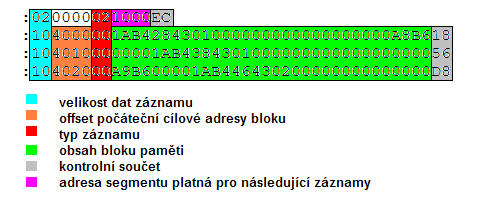
\includegraphics[trim=0cm 0cm 0cm 0cm, scale=0.7]{fig/intelhex}
\caption{Ukázka souboru ve formátu Intel HEX s popisky.}
\label{fig:intelhex}
\end{figure}

Formát Intel HEX pro MSP430 používá následující 4 typy záznamu:

\begin{itemize}
\item \textbf{00} - Datový záznam obsahující samotná data a 16bitovou adresu dat.
\item \textbf{01} - Konec souboru.
\item \textbf{02} - Rozšiřující segmentový záznam (MSB). Je používán pouze v případě, kdy je potřeba adresovat více než 16 bity.
\item \textbf{03} - Startovací záznam určující prvotní hodnotu PC registru (adresa daná jako segment (16 bitů) a offset (16 bitů); nejprve MSB)
\end{itemize}

\subsection{ELF}

Formát ELF (Executable and Linkable Format) je komplexní formát pro ukládání spustitelných souborů. Je rozšířen převážně na Unixových systémech. Formát ELF je základním výstupním formátem překladače GCC, který je často používán pro kompilování programů pro mikrokontroler MSP430. Kolem překladače GCC existuje řada dalších nástrojů, které umožňují získat z ELF souboru další informace aniž by musel programátor implementovat parser formátu ELF. \cite{elf}

Jedním z těchto nástrojů je program objcopy umožňující převod z ELF formátu do jiných formátů. Lze jím převést soubor z formátu ELF do formátu Intel HEX, který lze snadněji zpracovat. Dalším nástrojem je nástroj objdump. Pomocí tohoto nástroje lze například disassemblovat program obsažený v ELF souboru.

\subsubsection{DWARF - ladící informace}

Klíčovou vlastností formátu ELF je však možnost uložení ladících informací ve formátu DWARF. Popis DWARF formátu v této podkapitole vychází z \cite{dwarf}. Jedná se v podstatě o strom reprezentující celý výsledný
program. Jednotlivé části programu (zdrojové soubory, funkce, globální a lokální proměnné, datové typy atd.) jsou uzly tohoto stromu. Debuggery (jako je například GDB) pak těchto informací využívají při ladění programu a umožňují zobrazovat detailní ladící informace jako je hodnota lokální proměnné nebo zdrojový kód dané funkce.

\begin{figure}[ht]
\centering
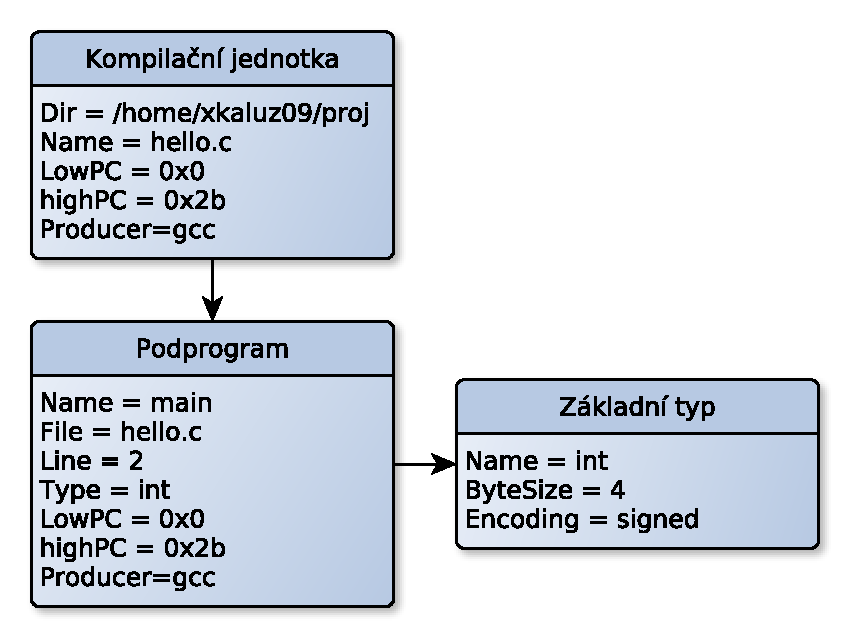
\includegraphics[trim=0cm 0cm 0cm 0cm, scale=0.7]{fig/dwarf}
\caption{DWARF strom Hello World programu v jazyce C.}
\label{fig:dwarf}
\end{figure}

Na obrázku \ref{fig:dwarf} lze vidět DWARF strom vygenerovaný pro jednoduchý program typu Hello World v jazyce C. Ze stromu je patrné, že každý uzel má svůj typ, od kterého se odvíjí jeho další atributy. Kořenem stromu je kompilační jednotka "hello.c" s atributy lowPC a highPC. Kdykoliv se vykonávání programu zastaví na instrukci s adresou mezi těmito dvěma atributy, jedná se o instrukci generovanou z této kompilační jednotky. V rámci této kompilační jednotky je definován pouze jediný podprogram "main" s návratovou hodnotou typu "int". Pokud by bylo podprogramů více, lze opět konkrétní podprogram určit za pomocí atributů lowPC a highPC a adresy aktuální instrukce. Datový typ "int" je definován jako základní znaménkový typ s velikostí 4 byty.

Formát DWARF definuje velké množství typů uzlů a jejich atributů. Z hlediska simulátorů je však důležité popsat ještě uložení proměnných. Proměnné mají kromě svého jména a typu ještě lokaci. Ta definuje, kde se nachází hodnota proměnné. Adresa proměnné se však může během běhu programu měnit - někdy bude výhodné mít proměnnou v registru, jindy v paměti, nebo dokonce z části v registru a z části v paměti. Proto je lokace proměnné ve formátu DWARF většinou definována v závislosti na adrese aktuální instrukce v takzvaném seznamu lokací.

Seznam lokací obsahuje pro každou proměnnou její lokaci v závislosti na adrese aktuální instrukce. Každá lokace je pak tvořena kódem zásobníkového automatu se speciálními mikroinstrukcemi, po jehož vykonání je na jeho vrcholu buď samotná hodnota proměnné, číslo registru ve kterém se hodnota nachází nebo
adresa místa v paměti, kde hodnotu najdeme.

K získání těchto informací z ELF souboru lze opět použít nástroj objdump.

\chapter{Událostně řízená simulace}

Udáje v této kapitole popisující událostně řízenou simulaci vychází z \cite{nutaro}.

Událostně řízená simulace modeluje simulovaný systém jako sled diskrétních událostí. Každá událost se odehrává v přesně stanoveném čase a mění celkový
stav systému. Mezi jednotlivými událostmi se stav systému nemění a je tak možné zpracovávat po sobě jdoucí události bez ohledu na časový interval
mezi nimi.

Každá událostně řízená simulace má svůj globální stav. Ten zahrnuje všechny proměnné a atributy studovaného systému. Globální stav se může v průběhu
simulace měnit vykonáváním událostí. Simulace také udržuje aktuální hodnotu simulačního času pro správné plánování událostí.

Další důležitou částí událostně řízené simulace je seznam událostí. V seznamu jsou události, které ještě nebyly zpracovány. Události jsou seřazeny
vzestupně podle simulačního času. Samotná simulace pak funguje tak, že simulátor změní simulační čas na hodnotu první naplánované události ze seznamu událostí. Tuto událost vykoná a pokračuje další naplánovanou událostí. Každá událost může při svém vykonávání přidávat do seznamu událostí další položky. Simulace končí při dosažení ukončující podmínky (například omezení simulačním časem nebo ukončení simulace při prázdném seznamu událostí).

\section{DEVS}

DEVS (Discrete Event System Specification) je hierarchický a modulární formalismus pro návrh a modelování systémů s diskrétními událostmi.
Základem DEVS je atomický model popisující chování části systému. Je definován jako sedmice:

\begin{math}
M=<X,Y,S,ta, \delta_{ext}, \delta_{int}, \lambda>
\end{math}

\begin{itemize}
\item $X$ - množina vstupních událostí.
\item $Y$ - množina výstupních událostí.
\item $S$ - množina stavů.
\item $ta:S \rightarrow \mathbb{T}^\infty$ - funkce posunu času definující dobu setrvání v daném stavu.
\item $\delta_{ext}:Q \times X \rightarrow  S$ - funkce změny stavu určující jak vstupní událost změní stav systému, kde $Q=\{(s,t_e)|s \in S, t_e \in (\mathbb{T} \cap [0, ta(s)])\}$ je množina všech stavů a $t_e$ je čas uběhlý od poslední události.
\item $\delta_{int}:S \rightarrow S$ je funkce definující změnu stavu systému po uplynutí doby setrvání v daném stavu.
\item $\lambda:S \rightarrow  Y^\phi$ je výstupní funkce, kde $Y^\phi=Y \cup \{\phi\}$ a $\phi \not\in Y$. Tato funkce definuje jak změna stavu systému, po uplynutí doby setrvání v něm, generuje výstupní událost.
\end{itemize}

Atomické modely tedy reagují na vstupní události změnou svého stavu a případně také generováním výstupní události. Svůj stav mohou měnit také samovolně po uplynutí doby setrvání v daném stavu.

Atomické modely je možné dále hiearchicky sdružovat pomocí formalismu Spojovaného DEVS definovaného jako osmice:

\begin{math}
N=<X,Y,D,\{M_i\},C_{xx}, C_{yx}, C_{yy}, Select>
\end{math}

\begin{itemize}
\item $X$ - množina vstupních událostí.
\item $Y$ - množina výstupních událostí.
\item $D$ - množina jmen podkomponent této DEVS komponenty.
\item $M_i$ - množina podkomponent kde pro každou platí $i \in D$.
\item $C_{xx}\subseteq X \times \bigcup_{i \in D} X_i$ - množina externích vstupních propojení.
\item $C_{yx}\subseteq \bigcup_{i \in D} Y_i \times \bigcup_{i \in D} X_i$ - množina interních propojení.
\item $C_{yy}: \bigcup_{i \in D} Y_i \rightarrow Y^\phi$ - množina externích výstupních propojení.
\item $Select:2^D \rightarrow D$ - množina funkcí určující jak vybrat událost z množiny událostí naplánovaných na stejný čas.
\end{itemize}

\chapter{Návrh událostně řízeného simulátoru}
\label{navrh}

Cílem této kapitoly je popsat strukturu navrženého simulátoru, jeho rozhraní pro komunikaci s periferiemi a mikrokontrolerem a knihovnu implementující mikrokontroler MSP430. Je zde také zmíněno grafické uživatelské rozhraní simulátoru.

\section{Struktura navrženého simulátoru}

Simulátor bude rozdělen do čtyř navzájem se dopňujících částí - simulační jádro, knihovna simulující MCU MSP430, komponenty rozšiřující simulační jádro a grafické uživatelské rozhraní.

Simulační jádro bude založeno na formalismu Spojovaného DEVS a bude umožňovat propojení všech simulovaných komponent. Komponenty budou atomickými modely formalismu DEVS a budou implementovat chování jednotlivých simulovaných periferií jako například tlačítka, LCD displeje nebo i samotného mikrokontroleru. Mikrokontroler bude vzhledem ke své komplexnosti implementován jako nezávislá knihovna. Grafické uživatelské rozhraní pak zpřístupní všechny funkce simulátoru uživateli.

\section{Návrh simulačního jádra}

Simulační jádro bude sloužit k řízení simulace, přeposílání zpráv mezi komponentami a umožní propojení simulovaných komponent (jednoho mikrokontroleru a více periferií). Každá komponenta bude samostatným modulem a bude mít pevně dané rozhraní pro komunikaci s jinými komponentami vyplývající z atomického modelu formalismu DEVS.

Vstupní a výstupní události definované ve formalismu DEVS budou chápány jako změny napětí na konkrétních pinech komponent. Propojení realizovaná pomocí Spojovaného DEVS pak budou reprezentovat propojení pinů komponent.

Každá komponenta bude schopna následujícího chování:

\begin{itemize}
\item Změnit svůj vnitřní stav na základě změny simulačního času - $ta$ funkce z definice formalismu DEVS.
\item Změnit svůj vnitřní stav na základě externí události přijaté na vstupní port (typicky na základě zprávy od jiné komponenty) - $\delta_{int}$ funkce z formalismu DEVS.
\item Generovat zprávy na výstupní port - $\lambda$ funkce z formalismu DEVS.
\end{itemize}

Mikrokontroler bude speciálním rozšířením běžné komponenty poskytujícím navíc přístup ke své paměti, regitrům a kódu programu. To umožní řídit simulaci na základě instrukcí a obsahu paměti a registrů daného mikrokontroléru. V rámci celé simulace bude jen jedna instance mikrokontroleru.

Simulační jádro bude umět komponenty dynamicky načítat aniž by docházelo k jeho jakékoliv úpravě. Návrh je tak velmi obecný a umožní snadné přidávání dalších rozšiřujících komponent nebo i simulaci jiného mikrokontroleru.

% \subsection{Komponenty}
% 
% Komponenta je nejmenší simulovatelná část systému. Komponenty jsou navrženy jako samostatné moduly s pevně daným rozhraním, pomocí kterého komunikují s ostatními komponentami simulace. Návrh je tak velmi obecný a umožňuje přidávání dalších rozšiřujících komponent.
% Návrh počítá se dvěma typy komponent:
% 
% \begin{itemize}
% \item \textbf{Periferie} - Je jakákoliv simulační komponenta, která umí reagovat na zprávy přijímané od jiných periférií, generovat nové zprávy a měnit svůj vnitřní stav na základě simulačního času.
% \item \textbf{Mikrokontroler (MCU)} - Jedná se o speciální případ periferie, která obsahuje paměť, registry a kód programu, který vykonává.
% To umožní řídit simulaci na základě instrukcí, obsahu paměti a registrů daného mikrokontroléru.  V rámci celé simulace je jen jedna instance mikrokontroleru. 
% \end{itemize}
% 
% Každá komponenta (periferie) tak bude schopna následujícího chování:
% 
% \begin{itemize}
% \item Změnit svůj vnitřní stav na základě změny simulačního času.
% \item Změnit svůj vnitřní stav na základě externí události přijaté na vstupní port (typicky na základě zprávy od jiné komponenty).
% \item Generovat zprávy na výstupní port.
% \end{itemize}
% 
% Mikrokontrolery navíc oproti periferiím budou poskytovat následující informace:
% 
% \begin{itemize}
% \item Obsah paměti a registrů.
% \item Disassemblovaný kód běžícího programu.
% \end{itemize}
% 
% Vstupní a výstupní porty definované ve formalismu DEVS budou představovat jednotlivé piny komponent. Spojení mezi porty pak bude značit spojení jednolivých
% pinů a zprávy posílané mezi porty budou reprezentovat aktuální napětí na pinech.

% Na obrázku .... lze vidět ukázku propojení dvou komponent (mikrokontroleru MSP430 a periferie - LED diody). Pokud program mikrokontroleru vygeneruje na svůj 
% výstupní port hodnotu 3.3 (tzv. 3.3 voltu), bude tato zprávy předána na vstupní port LED diody, která na jejím základě změní svůj vnitřní stav (tzv. rozsvítí se).

\section{Návrh knihovny simulující MCU MSP430}

Knihovna simulující mikrokontroler MSP430 je klíčovou částí projektu. Bude umožňovat nahrání uživatelského programu a jeho
následnou simulaci pomocí vykonávání instrukcí a běhu svých dalších interních komponent. Tato simulace bude řízena simulačním jádrem. Knihovna také poskytne grafickému uživatelskému rozhraní přístup ke své paměti a registrům, čímž umožní krokování programů. Bude také nabízet přístup k dalším ladícím informacím jako je například umístění lokálních a globálních proměnných v paměti nebo v registrech s využitím DWARF ladících informací.

Na obrázku \ref{fig:msp430_arch} lze vidět základní schéma MSP430 knihovny a její dekompozici. V této podkapitole jsou jednotlivé části tohoto schématu podrobněji rozebrány s důrazem na jejich funkci a postavení v rámci celé MSP430 knihovny.

\begin{figure}[ht]
\centering
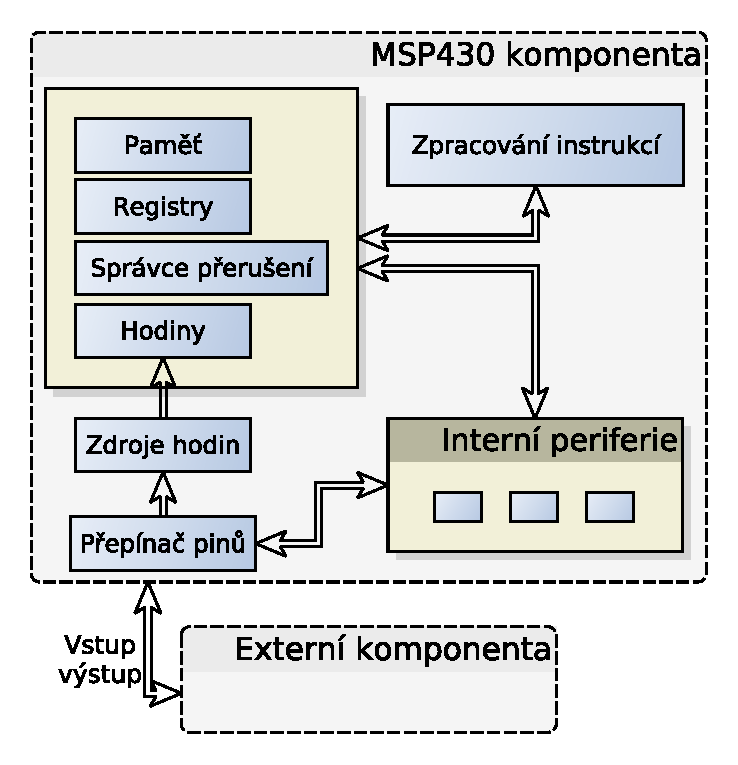
\includegraphics[trim=0cm 0cm 0cm 0cm, scale=0.7]{fig/msp430_arch}
\caption{Návrh architektury MSP430 komponenty.}
\label{fig:msp430_arch}
\end{figure}

\subsection{Paměť}

Paměť slouží k uchování jak uživatelského programu tak dat. Ostatní části mikrokontroleru (zejména pak interní periferie jako například USI nebo USCI) musí být schopny do paměti zapisovat jak slova tak jednotlivé byty a být informovány o případném čtení nebo zápisu provedeném uživatelským programem. To je podstatná vlastnost například pro automatické smazání příznaku přerušení po jeho přečtení. Dalším možným využitím informování o zápisu do paměti je možnost zastavení simulace po změně hodnoty v paměti a tím lepší možnost ladit uživatelský program.

Do paměti musí být umožněno načtení uživatelského programu ve formátu A43. Načítání programu z ELF souboru bude probíhat jeho převodem na formát A43 a následným načtením.

\subsection{Registry}

Návrh registrů, podobně jako návrh paměti, počítá s možností čtení a zápisu jednoho nebo dvou bytů. Opět je potřeba umožnit ostatním částem mikrokontroleru zjistit, že došlo k zápisu do registru. Typickým předpokládaným využitím je krokování programu na základě hodnoty PC registru. Další možné využití může být monitorování stavového registru a zastavení simulace při určitém příznaku.

\subsection{Přepínač pinů}

Každá varianta mikrokontroleru obsahuje různé interní periferie a tím pádem i jiný počet pinů a jejich rozmístění na pouzdru mikrokontroleru. Na jeden pin může být zapojeno více interních periferií a to, která periferie právě daný pin obsluhuje, je určeno na pomocí řídících registrů (například PxSEL a PxSEL2).

Jednotlivé varianty mikrokontroleru MSP430 budou z hlediska pinů a jejich připojení na interní periferie popsány v XML souboru, který bude obsahovat o každém pinu následující informace:

\begin{itemize}
\item Umístění pinu na pouzdru mikrokontroleru (vlevo, vpravo, ...) včetně jeho pořadí na dané straně pouzdra.
\item Seznam názvů vstupů/výstupů realizovaných pomocí pinu a hodnoty bitů v řídících registrech určujících, který vstup/výstup bude kdy zvolen.
\end{itemize}

Interní komponenty (například časovač nebo modul USI) budou mít zaregistrovány v přepínači pinů názvy svých vstupů a výstupů.
Přepínač pinů pak bude na základě aktuálně simulované varianty MSP430 mikrokontroleru monitorovat řídící registry PxSEL, PxSEL2, atd. a podle jejich hodnoty přeposílat vstupy z externích komponent konkrétním interním periferiím (princip multiplexoru). Tento princip ilustruje obrázek \ref{fig:msp430_pinmult}.

\begin{figure}[h]
\centering
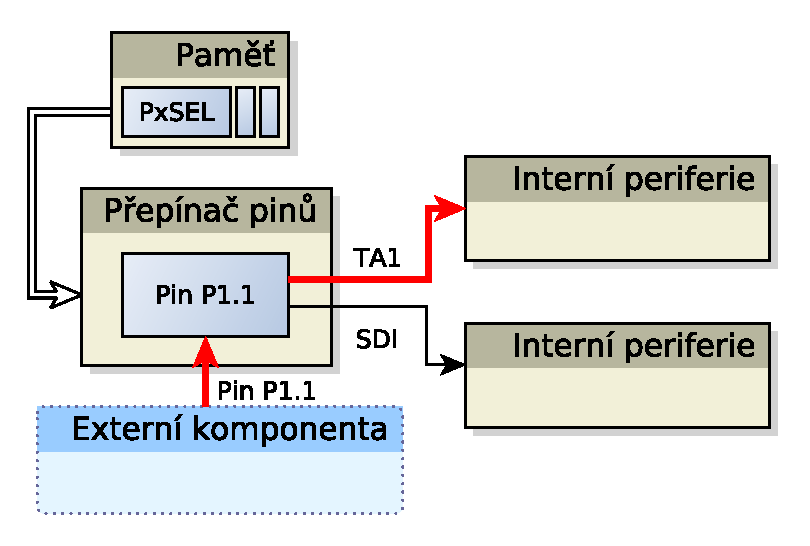
\includegraphics[trim=0cm 0cm 0cm 0cm, scale=0.7]{fig/msp430_pinmult}
\caption{Přepínač pinů přeposílá vstup z externí komponenty na interní periferii podle hodnoty PxSEL.}
\label{fig:msp430_pinmult}
\end{figure}

Přepínač pinů bude rovněž směrovat signály uvnitř MSP430 komponenty. Toho bude potřeba pro interní propojení jednotlivých interních periferií (například výstup časovače může být použit jako vstup modulu USI - toto propojení se děje uvnitř MSP430 komponenty bez využití externích pinů).

\subsection{Zdroje hodin}

Zdroje hodin budou generovat hodinový signál o určité frekvenci. Tento signál pak bude sloužit hodinám (MCLK, SMCLK a ACLK) pro řízení jednotlivých částí mikrokontroleru. Z hlediska simulace je možné zdroje hodin rozdělit na dvě kategorie. Zdroje závislé na externích komponentách (LFXT1CLK, XT2CLK) a zdroje závislé pouze na čase (VLOCLK, DCOCLK).

Zdroje závislé na externích komponentách musí být schopny přijímat zprávy od externích komponent a na jejich základě pak generovat hodinový signál, který je dále zpracován jednotlivými hodinami.

Zdroje závislé na čase musí být samostatnými simulačními komponentami a musí samy na základě uběhnutého času generovat hodinový signál s patřičnou frekvencí.

Všechny zdroje hodin musí generovat informace jak o náběžné, tak o sestupné hraně hodinového signálu. To je podstatná vlastnost například pro modul USI, který provádí své akce jak s oběma hranami hodinového signálu.

\subsection{Hodiny}

Hodiny (MCLK, SMCLK a ACLK) dále zpracovávají hodinový signál od zdrojů hodinového signálu. Umožňují nastavit děličku, čímž mění frekcenci hodinového signálu. K jednotlivým hodinám budou připojeny interní periferie, které jimi budou řízeny. Stejně jako u zdrojů hodinového signálu je potřeba u zdrojů hodin poskytovat informace jak o náběžné tak o sestupné hraně.

\subsection{Správce přerušení}

Správce přerušení bude udržovat informace o požadavcích na přerušení. Modulu zpracovávajícímu instrukce umožní spustit rutinu přerušení, pokud je nějaké
přerušení ve frontě. Ostatním interním komponentám pak umožní žádat o přerušení.

Interní komponenty budou rovněž potřebovat informaci o dokončení konkrétního typu přerušení (například pro vymazání příznaku přerušení po jeho obsluze).

\subsection{Zpracování instrukcí}

Zpracování instrukcí ilustruje diagram na obrázku \ref{fig:msp430_inst}.

\begin{figure}[h]
\centering
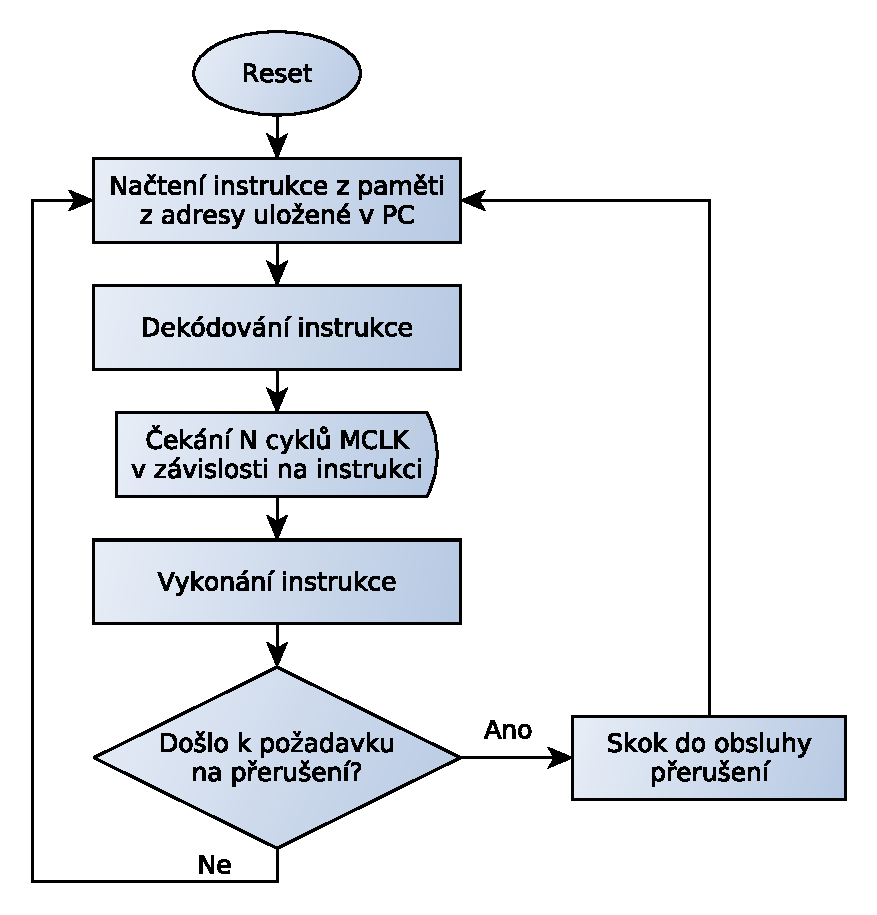
\includegraphics[trim=0cm 0cm 0cm 0cm, scale=0.7]{fig/msp430_inst}
\caption{Diagram zpracování instrukcí.}
\label{fig:msp430_inst}
\end{figure}

Z obrázku lze vidět, že je zpracování instrukce rozděleno na několik částí. Nejprve je instrukce načtena z paměti v závislosti na hodnotě registru PC (R0).
Dále dojde k dekódování instrukce a jejímu vykonání. Vykonání instrukce je atomické a trvá několik MCLK cyklů. Počet cyklů potřebných pro vykonání
instrukce je znám již po jejím dekódování. Proto je mezi dekódováním a vykonáním vloženo čekání simulující vykonávání instrukce na reálném HW.
Po vykonání instrukce je potřeba obsloužit jakákoliv přerušení, která mohla v mezičase nastat. Tento cyklus se bude opakovat stále dokola, dokud MCLK generuje další pulsy (tzv. dokud simulace běží).

\subsection{Interní periferie}

Interní periferie budou využívat modulů popsaných dříve v této kapitole. Každá interní periferie tak bude mít přístup k paměti, registrům, pinům, správci
přerušení a hodinovému signálu. V rámci diplomové práce bude z interních periferií implementován časovač, modul USI a USCI.

Jako příklad návrhu interní periferie se tato podkapitola věnuje pouze časovači. Princip návrhu ostatních periferií je však obdobný, liší se pouze jejich funkcí.

\subsubsection{Časovač}

Časovač bude monitorovat své řídící registry prostřednictvím paměťového modulu a v případě jejich změny, způsobené uživatelským programem, změní také své nastavení (výběr módu, vstupů atd.). Pro generování nastavení Capture overflow bitu (indikace situace, kdy uživatelský program nestihl přečíst hodnotu časovače během 2 přerušení) je potřeba vědět, zda uživatelský program přečetl aktuální hodnotu časovače. To bude řešeno opět pomocí paměťového modulu, kdy tento bude informovat časovač o přečtení dané hodnoty z paměti.

Časovač musí být schopen zvyšovat svoji hodnotu v závislosti na frekvenci. Proto bude časovač napojen na modul hodin (SMLK nebo ACLK). S každým cyklem
hodin pak v závislosti na svém nastavení vykoná danou funkci.

Pomocí časovače lze rovněž generovat pulsy na výstupních pinech umístěných na pouzdře mikrokontroleru a vzorkovat napětí na pinech vstupních.
Je proto nutné umožnit časovači přístup k těmto pinům. To bude provedeno pomocí přepínače pinů. Časovač si zaregistruje potřebné názvy vstupů a výstupů
a přepínač pinů pak v závislosti na akcích uživatelského programu bude směrovat vstupy mikrokontroleru přímo do časovače.

Přerušení časovače jsou generována pomocí správce přerušení. Je však potřeba zajistit, aby se časovač dozvěděl o dokončení rutiny obsluhující přerušení
(přerušení časovače je sdíleno více zdroji přerušení a časovač musí být schopen požádat o další přerušení z jiného zdroje ihned po obsloužení původního přerušení). Toto je zajištěno monitorováním ukončených přerušení pomocí správce přerušení.

Z příkladu časovače lze vidět, že návrh a dekompozice mikrokontroleru MSP430 je dostačující pro interní periferie a poskytuje všechny potřebné vlastnosti.

\section{Návrh grafického uživatelského rozhraní}

Hlavní funkcí grafického uživatelského rozhraní bude řízení simulace, jednoduchá editace jednotlivých simulovaných komponent a ladění programu mikrokontroleru.

Grafické uživatelské rozhraní by tedy mělo mít následující funkce:

\begin{itemize}
\item \textbf{Správa projektu} - Vytvoření, uložení a nahrání projektu.
\item \textbf{Editace projektu} - Přidávání a odebírání simulovaných komponent a editace jejich propojení.
\item \textbf{Řízení simulace} - Nastavení parametrů simulace, kontrola jejího běhu, krokování atd.
\item \textbf{Ladění programu} - Zobrazení zdrojového kódu programu, hodnoty proměnných, registrů, paměti.
\item \textbf{Ladění signálů} - Možnost kontrolovat v čase signály přenášené mezi simulovanými komponentami.
\end{itemize}

V této kapitole jsou tyto požadavky kladené na grafické uživatelské rozhraní detailně rozebrány a je navrženo grafické uživatelské rozhraní, které tyto
požadavky splňuje.

\subsection{Základní koncepce}

Nejdůležitější součástí hlavního okna simulátoru bude kreslící plocha. Na této ploše budou vykresleny jednotlivé simulované komponenty (mikrokontroler
a periferie) včetně jejich pinů a propojení mezi piny. Uživatel bude schopen přidávat nové komponenty a odstraňovat stávající, propojovat je pomocí
vodičů a měnit jejich vlastnosti (například barvu LED diody). Během simulace se budou všechny komponenty aktualizovat a uživatel tak uvidí průběh simulace
(LED dioda bude blikat, aktivní piny budou zobrazeny rozdílnou barvou než piny neaktivní atd.).

Další důležitou částí grafického uživatelského rozhraní bude zobrazení zdrojového kódu programu nahraného v mikrokontroleru. Tento kód bude poskytnut
přímo mikrokontrolerem a GUI jej pouze zobrazí. Z principu lze vždy zobrazit kód v assembleru. Pokud však bude dostupný zdrojový kód v jazyce C, bude 
simulátor schopen přepínat mezi kódem v assembleru a kódem v C. Po zastavení simulace se zobrazí aktuální instrukce (případně odpovídající příkaz v jazyce C). Uživatelské rozhraní bude rovněž umožňovat nastavení breakpointů (bodů zastavení) na jednotlivých instrukcích, čímž umožní jednodušší krokování
simulace.

Pro zobrazení interních informací o jednotlivých simulovaných komponentách bude sloužit třetí část uživatelského rozhraní. Půjde o strukturovaný seznam
typu název-hodnota, který bude zobrazovat informace o aktuálních hodnotách registrech mikroprocesoru, důležitých místech v paměti, nebo například hodnotách
lokálních proměnných v místě zastavení simulace. Každá komponenta bude schopna přidat do tohoto seznamu své položky a předávat tak uživateli potřebné
interní informace.

Poslední dílčí částí uživatelského rozhraní bude rozhraní pro zobrazení napětí na jednotlivých pinech formou osciloskopu. Uživatel si bude moci vybrat
piny, které chce během simulace sledovat a během simulace (nebo i po jejím zastavení) uvidí veškeré změny signálu, které se na pinech odehrály.

\subsection{Správa projektu}

Při vytvoření nového projektu bude uživatel dotázán na vybrání jeho architektury (návrh celé aplikace se neomezuje pouze na mikrokontrolery rodiny MSP430) a varianty dané architektury (v případě mikrokontroleru MSP430 se bude jednat o jeho konkrétní typ). Po vytvoření projektu uvidí uživatel na kreslící ploše vybraný mikrokotroler a bude mu umožněno nahrání programu a přidání dalších periferií.

Při uložení projektu bude potřeba uložit informace o všech komponentách, jejich propojení a umístení na kreslící ploše. Budou se rovněž ukládat informace
o aktuálně používaných breakpointech a sledovaných pinech.

\subsection{Editace projektu}

Editace projektu bude probíhat na kreslící ploše zobrazující všechny komponenty. Na kreslící plochu bude možné přidávat nové periferie ze seznamu periferií, případně ostraňovat periferie stávající. Uživateli bude umožněno periferiemi volně pohybovat po kreslící ploše a propojovat jejich piny pomocí vodičů. Bude možné propojit i více než 2 piny (lze tak vytvořit sběrnicovou topologii s uzly). Propojení mezi piny bude možné odstraňovat.

\subsection{Řízení simulace}

Grafické uživatelské rozhraní umožní spuštění simulace, její dočasné zastavení a její restartování. Během simulace bude uživateli prezentován aktuální simulační čas a uvidí změny simulovaného zapojení na kreslící ploše a osciloskopu. Při dočasném zastavení simulace uvidí uživatel aktuální
stav simulovaného zapojení (stav všech registrů a paměti, následující instrukci ve zdrojovém kódu atd.). Simulaci bude také možné automaticky zastavit po určitém simulačním čase.

K dispozici bude také funkce pro krokování programu s následujícími 3 módy:

\begin{itemize}
\item \textbf{Událost simulace} - Provede další událost v simulaci. Jedná se například o jeden tik hodin MCLK, nebo 1 tik externího oscilátoru. Jedna událost je nejmenší možný krok, jaký lze v diskrétní simulaci provést.
\item \textbf{Instrukce} - Provede další instrukci mikrokontroleru. Instrukce zpravidla trvá více simulačních kroků, půjde tedy o méně jemné krokování simulace.
\item \textbf{Řádek v jazyce C} - Provádí instrukce mikrokontroleru, dokud tyto implementují stále tentýž řádek ve zdrojovém souboru v jazyce C. Při volbě tohoto krokování musí být výsledná aplikace schopna detekovat cykly (například 1 instrukce NOP opakující se stále dokola ve smyčce), aby nedošlo k zamrznutí simulace při vykonávání kroku.
\end{itemize}

Další možností pozastavení simulace jsou takzvané breakpointy. Uživatel musí umět nastavit pozastavení simulace v případě, kdy určitý registr nabyl jím definovanou hodnotu (případně když hodnota v paměti definovaná adresou nabyla konkrétní hodnotu).

\subsection{Ladění programu}

Při každém pozastavení simulace uvidí uživatel aktuální instrukci ve zdrojovém kóu. Kromě samotného zdrojového kódu mu budou zobrazeny, pokud byl nahrán program ve formátu ELF s ladícími symboly, názvy všech zdrojových souborů nahraného programu a všech funkcí v daných souborech. Uživatel bude moci vybrat daný soubor a funkci v něm pro rychlejší orientaci v projektu. V případě dostupnosti zdrojového kódu v jazyce C se uživateli zobrazí jeho kód. Vždy však bude možné zobrazit diassemblovaný kód v assembleru. Uživatel bude moci přidávat breakpointy v libovolných místech kódu a po opětovném spuštění simulace se tato zastaví na místě, které uživatel zvolil.

V grafickém uživatelském rozhraní budou rovněž zobrazeny hodnoty registrů a důležitých adres v paměti (standardně hexadecimálně, avšak bude možné zobrazit jejich hodnoty i v jiných soustavách). Uživatel bude moci použít tento seznam registrů a míst v paměti pro rychlé přidání nových breakpointů. Na základě místa ve zdrojovém kódu, na kterém došlo k pozastavení simulace, budou zobrazeny jména a hodnoty lokálních proměnných.

\subsection{Ladění signálů}

Uživateli bude umožněno vybrání pinů na kreslící ploše a jejich zařazení do seznamu sledovaných pinů. V pruběhu simulace se změny napětí na sledovaných pinech budou ukládat a zobrazovat uživateli v graficky pomocí rozhraní podobného osciloskopu. Uživatel tak uvidí vztahy mezi jednotlivými signály generovanými na pinech v závislosti na čase. Standardně bude rozhraní ukazovat průběh celé simulace. Bude však možné určitý časový úsek přiblížit a získat tak detailnější pohled. Uživatelské rozhraní rovněž umožní export těchto dat.

\chapter{Implementace}

Cílem této kapitoly je popsat výsledný implementovaný simulátor založený na předešlém návrhu. Jako výchozí jazyk byl zvolen jazyk C++. Jedná se o jazyk podporující objektově orientované programování (OOP), čímž zjednodušuje dekompozici celého projektu na menší celky. Nástroj QDevKit, který může v budoucnu implementovaný simulátor rozšířit, je rovněž programován v jazyce C++, takže bude jejich budoucí spravování jednodušší.

Pro tvorbu grafického uživatelského rozhraní byla použita knihovna Qt. Jedná se o multiplatformní knihovnu použitou i v projektu QDevKit licencovanou pod licencí LGPL.

V následujících kapitolách jsou popsány implementační detaily jednotlivých částí simulátoru. Vzhledem k rozsáhlosti celého projektu se tato kapitola soustředí pouze na nejzajímavější aspekty implementace a nepopisuje implementaci do úplných detailů.

\section{Implementace simulačního jádra}

Jako základ pro simulační jádro byla použita knihovna ADEVS. Tato knihovna implementuje diskrétní simulaci formalismem DEVS a je šířena pod licencí GPLv2+. Díky této licenci může být použita i v případě bližší integrace simulátoru do prostředí QDevKit.

\subsection{Knihovna ADEVS a její využití}

Hlavní třídou knihovny ADEVS je třída adevs::Simulator. Tato třída určuje typ událostí, které se mezi jednotlivými simulovanými komponentami přeposílají a umožňuje řídit simulaci (lze například získat čas následující události a vykonat ji). Mezi komponentami se posílají události typu double (desetinné číslo),  které určují velikost napětí. Existuje zde však také speciální hodnota, která určuje stav vysoké impedance - DBL\_MAX.

Atomické modely formalismu DEVS jsou reprezentovány třídou adevs::Atomic. Tato třída obsahuje následující metody známé z formalismu DEVS:

\begin{itemize}
\item \textbf{delta\_int(...)} - metoda volána v případě změny interního stavu modelu.
\item \textbf{delta\_ext(...)} - metoda volána v případě externí události generované jiným modelem.
\item \textbf{output\_func(...)} - metoda volána v případě, kdy má model vygenerovat své výstupní události.
\item \textbf{ta(...)} - metoda určující čas setrvání v aktuálním stavu.
\end{itemize}

Každá simulovaná komponenta tak musí být dceřinou třídou třídy adevs::Atomic. Při spuštění (nebo restartování simulace) se musí veškeré komponenty a jejich propojení vytvořit znovu, protože mohly být v grafickém uživatelském rozhraní přidány nové komponenty a změněny jejich dosavadní propojení. To představuje problém, protože komponenta není tvořena pouze simulační částí (tzv. třídou adevs::Atomic), ale i mnoha dalšími třídami, jejichž chování dědí (je například nutné komponenty vykreslovat v grafickém uživatelské rozhraní - dědit tomu odpovídající třídu). Není však optimální vytvářet objekty v grafickém uživatelském rozhraní znovu při každém restartování simulace.

Tento problém byl vyřešen oddělením simulační části komponenty do samostatné třídy SimulationObjectWrapper dědící ze třídy adevs::Atomic a využívající návrhový vzor Proxy. Tato třída mapuje volání metod třídy adevs::Atomic na volání třídy SimulationObject, ze které pak všechny simulované komponenty dědí
své chování. Tento vztah znázorňuje obrázek \ref{fig:adevs_classes} Při restartování simulace tak nemusí být smazána a znovu vytvořena celá komponenta (třída SimulationObject), ale pouze třída SimulationObjectWrapper.

Třída adevs::Simulator potřebuje ke svému běhu také instanci třídy adevs::Network. Tato třída reprezentuje formalismus Spojovaného DEVS a definuje sadu čistě virtuálních metod, které pak dceřiné třídy implementují (například pomocí metody route(...) se směrují události mezi komponentami). Knihovna ADEVS obsahuje několik implementací této třídy. Bohužel jsou však tyto implementace velmi obecné a tím pádem i pomalé. Bylo tak nutné vytvořit novou třídu SimulationModel, která pracuje přímo s objekty typu SimulationObjectWrapper.

\subsection{Rozšiřitelné periferie formou modulů}

Jak již bylo zmíněno v předchozí podkapitole, každá simulovaná komponenta je dceřinou třídou třídy SimulationObject. Rozšiřitelné moduly umožňují načtení implementace této třídy ze sdílené knihovny nebo z kódu modulu v jazyce Python. Protože je každou komponentu potřeba vykreslit v grafickém uživatelském rozhraní a umožnit interakci uživatele, musí rozšiřitelný modul implementovat rovněž třídu ScreenObject (tato je popsána dále v kapitole TODO). Pro jednoduchost byly tyto dvě třídy zapouzdřeny v třídě Peripheral, která je výslednou třídou pro implementaci rozšiřitelných modulů. Vztahy mezi popsanými třídami je možné vidět na obrázku \ref{fig:adevs_classes}

\begin{figure}[ht]
\centering
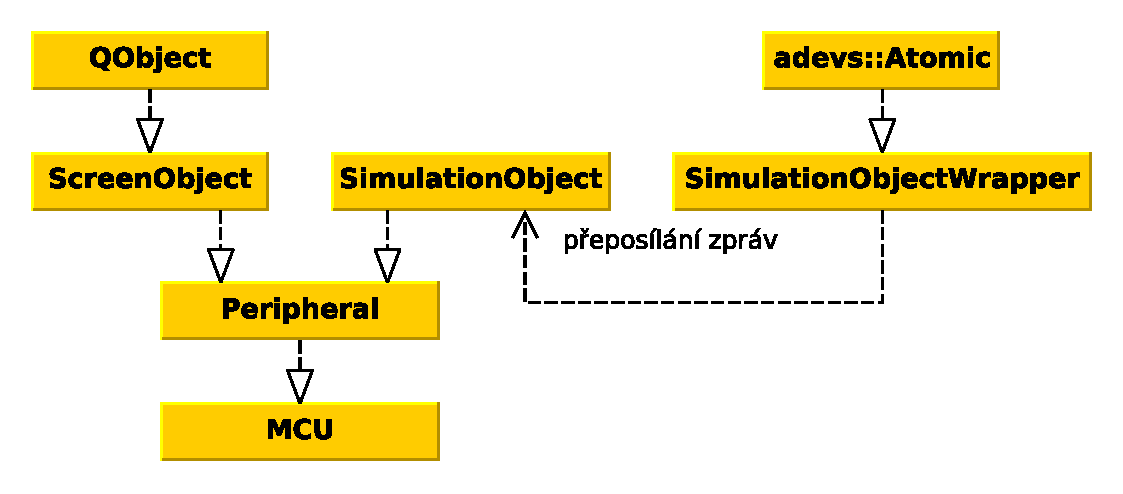
\includegraphics[trim=0cm 0cm 0cm 0cm, scale=0.7]{fig/adevs_class}
\caption{Diagram znázorňující vztahy mezi třídami knihovny ADEVS, simulovanými periferiemi a mikrokontrolery.}
\label{fig:adevs_classes}
\end{figure}

Každý modul obsahuje XML soubor obsahující jeho metadata. Jedná se zejména o jméno modulu, jméno autora, typ modulu (Pyhon nebo dynamická knihovna), název knihovny a licence. Tento XML soubor je načten třídou PeripheralManager a na základě metadat je pak dále nahrán jeho kód. Nahrání kódu modulu se liší v závislosti na typu modulu a je popsáno v následujících dvou podkapitolách.

Na základě metadat a nahraného kódu modulu je vytvořena instance třídy PeripheralInfo, kterou pak využívají další části simulátoru. Tato třída obsahuje metodu pro vytvoření nové instance periferie a poskytuje o periferii základní informace (například jméno). Seznam všech nahraných modulů lze pak získat pomocí již zmíněné třídy PeripheralManager.

\subsubsection{Moduly v jazyce C++}

Moduly naprogramované v jazyce C++ jsou načítány jako sdílené knihovny pomocí třídy QPluginLoader poskytované knihovnou Qt. Při programování C++ modulů je potřeba kromě třídy Peripheral implementovat rovněž třídu PeripheralInterface (s jedinou metodou create(...)), která slouží pro vytváření nových instancí periferií a kterou QPluginLoader používá k identifikaci modulu.

Ukázku kódu v jazyce C++ implementující jednoduché periferie lze najít v kapitole TODO.

\subsubsection{Moduly v jazyce Python}

Pro vytváření modulů v jazyce Python je využita knihovna PythonQt. Tato knihovna poskytuje rozhraní mezi Qt knihovnou a jazykem Python. Je rovněž použita v projektu QDevKit a tak při případné distribuci obou aplikací současně není přidávána žádná nová závislost.

Základ pro tvorbu modulů v jazyce Python byl převzat z projektu QDevKit (jedná se o třídy Script a ScriptEngine), avšak byly provedeny výkonostní optimalizace.

Pomocí třídy ScriptEngine jsou načteny moduly v jazyce Python třídou PeripheralManager a jsou dále reprezentovány jako instance třídy Script. Nad třídou Script jsou implementovány třídy PythonPeripheralInterface (rozšiřující třídu PeripheralInterface) a PythonPeripheral (rozšiřující třídu Peripheral).

Třída PythonPeripheralInterface vytváří novou instanci třídy PythonPeripheral, čím vznikne nová periferie. Třída PythonPeripheral dědí rozhraní třídy Peripheral a mapuje všechna její volání pomocí knihovny PythonQt do jazyka Python.

Ukázka kódu v jazyce Python implementující jednoduché periferie je rovněž popsána dále v kapitole TODO.

\subsection{Rozšiřitelné MCU formou modulů}

Jádro simulátoru rovněž umožňuje implementaci jiných 16 bitových mikrokontrolerů. Tyto mikrokontrolery mohou být načítány pouze jako sdílené knihovny naprogramované v jazyce C++. Mikrokontroler je reprezentován třídou MCU (rozšiřuje třídu Peripheral), která musí být děděna každým mikrokontrolerem.

Třída MCU rozšiřuje třídu Peripheral zejména o možnost přístupu k paměti a registrům mikrokontroleru a přistupu k ladícím informacím pro aktuální program (viz podkapitola TODO).

Paměť MCU je reprezentována třídou Memory, obsahující základní metody pro změnu paměťových buněk (setByte(...), getByte(...) atd.). Umožňuje také nastavit paměťové buňce instanci třídy MemoryWatcher, jejíž metoda handleMemoryChanged(...) (případně handleMemoryRead(...)) je volána pokud došlo ke změně hodnoty na této adrese.

Registry mikrokontroleru jsou zapouzdřeny ve třídě RegisterSet. Každý register je tvořen třídou Register, která rovněž poskytuje metody k jeho změně a nabízí možnost jeho sledování pomocí instance třídy RegisterWatcher.

Načítání modulů mikrokontrolerů funguje obdobně jako u periferií. Existují zde analogické třídy MCUInterface, MCUManager a MCUInfo.

\subsection{Podpora breakpointů}

Breakpointy umožňují zastavení simulace v případě splnění určíté, předem dané, podmínky. Byly implementovány dva typy breakpointů - zastavení simulace v případě změny hodnoty registru a zastavení simulace v případě změny hodnoty pamětí na určité adrese.

V obou případech slouží pro registraci breakpointů třída BreakpointManager. Tato třída využívá tříd RegisterWatcher a MemoryWatcher ke sledování registrů a paměti a v případě splnění podmínky breakpointu zastaví simulaci.

V případě zastavení simulace na základě hodnoty registru je jedním z nejčastějších případě zastavení na základě hodnoty registru PC. Tohoto se využívá pro krokování programu nebo jeho zastavení na určité instrukci. Je nutné umožnit nastavení více hodnot jednoho registru jako podmínky pro zastavení simulace. 

Jelikož ke změně hodnoty registrů dochází velmi často, je potřeba zjistit velmi rychle, zda-li je aktuální hodnota registru důvodem k zastavení simulace. Pro každý registr je uložen seznam všech breakpointů (hodnot registrů). Tento seznam je při vložení nové hodnoty seřazen algoritmem quick sort a pro vyhledání hodnoty v seznamu je využito binární vyhledávání.

V případě zastavení simulace na základě hodnoty v paměti je navíc umožněno zastavit simulaci v případě jakékoliv změny paměti a implementace počítá s možným budoucím rozšířením o složitější podmínky (například příslušnost hodnoty v daném rozsahu nebo změna konkrétního bitu na dané adrese).

\section{Implementace zpracování DWARF informací}

Aby bylo možné při ladění programu získat hodnoty a typ lokálních proměnných, je potřeba načítat a zpracovávat DWARF ladící informace. Pro samotné uchování jednotlivých struktur formátu DWARF byly vytvořeny následující abstraktní třídy (jejich vztahy lze vidět na obrázku \ref{fig:dwarf_classes}):

\begin{itemize}
\item \textbf{VariableType} - Třída reprezentující typ proměnné uložené v DWARF informacích. Obsahuje informace jako je například název typu ("int", "char *", ...), velikost typu v bytech, způsob zakódování v paměti nebo například podtyp (v případě že jde o pole prvků jiného typu).
\item \textbf{VariableValuePiece} - Třída obsahující informaci o umístění části hodnoty proměnné v paměti nebo registrech mikrokontroleru. Hodnoty proměnných mohou být rozděleny na části například v případě, kdy část hodnoty proměnné je umístěna v registrech a část v paměti.
\item \textbf{VariableValue} - Pole instancí tříd VariableValuePiece, které reprezentuje kompletní hodnotu dané proměnné.
\item \textbf{Variable} - Třída zapouzdřující třídy VariableType a VariableValue definující jednu proměnnou daného programu.
\item \textbf{Subprogram} - Třída definující podprogram. Obsahuje seznam lokálních proměnných a argumentů podprogramu (instancí tříd Variable), jeho jméno a rozsah paměti, na které se kód podprogramu nachází
\item \textbf{DebugData} - Hlavní třída reprezentující kompletní DWARF ladící informace daného programu. Obsahuje seznam všech podprogramů (instancí tříd Subprogram).
\end{itemize}

Tyto třídy jsou obecnými třídami pro uchování ladících informací a nejsou nikterak přímo závislé na využítí formátu DWARF. V rámci této diplomové práce je však zpracováván pouze formát DWARF. Pro uložení dalších potřebných informací specifických pro formát DWARF bylo potřeba definovat ještě následující 3 třídy:

\begin{itemize}
\item \textbf{DwarfExpression} - Třída obsahující kód mikroinstrukcí pro zásobníkový automat definovaný formátem DWARF pro získání hodnoty proměnné (nebo její adresy) v závislosti na aktuálně zpracovávané instrukci. Tato třída zmíněný zásobníkový automat rovněž implementuje.
\item \textbf{DwarfLocation} - Třída zapouzdřující třídu DwarfExpression a definující rozsah adres, pro který je kód uložený v DwarfExpression platný.
\item \textbf{DwarfLocationList} - Seznam instancí tříd DwarfLocation.
\end{itemize}

Načtení DWARF ladících informací probíha za pomocí třídy DWARFLoader. Tato třída využívá nástroje objdump dodávaného s překladačem GCC. Nástroj objdump je postupně spuštěn s přepínači "--dwarf=info" a "--dwarf=loc", jejichž výstup je touto třídou rozparsován a zpracován a jsou vytvořeny instance výše zmíněných tříd.

\subsection{Využití DWARF informací}

Jedním z příkladu využití DWARF ladících informací je zobrazení lokálních proměnných aktuálně prováděného podprogramu. Při zastavení simulace na určité instrukci je za pomocí její adresy (hodnoty registru PC) nalezen aktuálně prováděný podprogram prostřednictvím třídy DebugData. Z podprogramu (instance třídy Subprogram) je získán seznam lokálních proměnných a pro každou proměnnou (instanci třídy Variable) je zavolána funkce pro získání její hodnoty.

Pokud není hodnota proměnné závislá na hodnotě registru PC, obsahuje instance třídy Variable přímo instanci třídy DwarfExpression. V opačném případě je v seznamu lokací DwarfLocationList nalezena odpovídající instance třídy DwarfExpression (na základě hodnoty registru PC). Dále je vyhodnocen kód zásobníkového automatu uloženého ve zmíněné třídě DwarfExpression a na základě výsledku je určena hodnota proměnné.

Hodnotu proměnné je potřeba reprezentovat odpovídajícím způsobem v závislosti na jejím typu. K tomu slouží třída VariableFormatter, která na základě typu proměnné formátuje její hodnotu a vrátí ji jako řetětec znaků.

\section{Implementace knihovny simulující MCU MSP430}

Knihovna simulující MCU MSP430 vykonává instrukce simulovaného programu a poskytuje všechny interní moduly poskytované mikrokontrolerem.

Hlavní třídou knihovny je třída MCU\_MSP430, která reprezentuje celý mikrokontroler. V této třídě jsou vytvářeny a navzájem propojeny jednotlivé dílčí podtřídy, kterými se dále tato kapitola zabývá. Třída MCU\_MSP430 dědí ze třídy MCU a lze ji tak přímo použít jako rozšiřující modul simulátoru.

Nejjednoduššími třídami simulátoru jsou třídy Memory, RegisterSet a Register. Třída Memory implementuje paměť jako pole bytů a umožňuje její čtení a zápis včetně informování o změně jednotlivých bytů pomocí instance třídy MemoryWatcher. Obdobně jsou implementovány třídy RegisterSet a Register.

\subsection{Implementace jednotlivých variant MCU MSP430}

Implementace knihovny umožňuje simulování většiny podporovaných variant mikrokontroleru MSP430. Každá varianta mikrokontroleru MSP430 je reprezentována vlastní třídou dědící ze třídy Variant. Tyto třídy jsou vytvořeny při načtení knihovny a lze k nim přistupovat na základě řetězce udávajícího název varianty funkcí getVariant(...).

Třída Variant obsahuje metody pro získání informací, které jsou pro dané varianty specifické. Jedná se například o adresy jednotlivých portů (metoda getP1DIR()), indexy vektorů přerušení (například metoda getUSART1TX\_VECTOR()) nebo například získání počáteční adresy vektoru přerušení (metoda getINTVECT()).

Vytváření těchto tříd ručně podle dokumentace by bylo značně obtížné a byl proto zvolen lepší přístup. Kompilátor msp430gcc obsahuje pro každou variantu mikrokontroleru hlavičkový soubor definující jednotlivé údaje specifické pro daný mikrokontroler a jeho vlastnosti. Byl vytvořen skript v jazyce Python, kterým lze za použití nástroje msp430-gcc s přepínači -E a -dM získat z tohoto hlavičkového souboru seznam všech těchto definic pro daný mikrokontroler.

Tento seznam je pak dále zpracován a jsou z něj vybrány pouze ty definice, které jsou v knihovně simulující MCU MSP430 potřeba. Následně je vygenerována samotná třída Variant a i všechny její implementace - pro každý mikrokontroler jedna.

Tímto postupem byla jednoduše vyřešena většina rozdílů mezi variantami mikrokotrolerů včetně detekce různých interních modulů poskytovaných různými variantami.

\subsection{Načítání programu}

Pomocí knihovny lze načítat programy pro miktrokontroler ve formátu ELF a Intel HEX (A43). Načítání souborů ve formátu A43 provádí metoda loadA43(...) třídy Memory. Tato metoda rozparsuje data ve formátu A43, uloží je na dané místo v paměti a nastaví registr PC na adresu první instrukce.

Načítání souborů ve formátu ELF probíhá s využitím pomocné třídy CodeUtil. Ta za pomocí nástroje msp430-objcopy převede program z formátu ELF do formátu A43, který je pak možné načíst pomocí třídy Memory.

Při načítání programu je program rovněž disassemblován. To je provedeno pomocí nástroje msp430-objdump, jehož výstup je rozparsován a dále zpracováván grafickým uživatelským rozhraním.

\subsection{Dekódování a vykonávání instrukcí}

Instrukce je reprezentována instancí třídy Instruction. Tato třída uchovává informace o zdrojovém a cílovem argumentu instrukce, o jejím typu, offsetu a případném bytovém módu. Každý argument je uložen jako implementace abstraktní třídy InstructionArgument definující základní rozhraní pro každý argumentu. Byly implementovány následující typy argumentů:

\begin{itemize}
\item \textbf{ConstantArgument} - Argumentem je konstanta.
\item \textbf{MemoryArgument} - Argumentem je místo v paměti dané adresou.
\item \textbf{IndexedArgument} - Argumentem je místo v paměti dané adresou a offsetem.
\item \textbf{IndirectAutoincrementArgument} - Argumentem je místo v paměti dané adresou uloženou v registru, která je po vykonání instrukce inkrementována.
\item \textbf{Register} - Registr může být také argumentem instrukce a tak již dříve zmíněná třída Register rovněž implementuje třídu InstructionArgument.
\end{itemize}

Instrukce jsou dekódovány pomocí třídy InstructionDecoder. Tato třída načte aktuální instrukci z paměti, rozparsuje ji, uloží do instance třídy Instruction a vrací počet hodinových cyklů potřebných k těmto úkonům. Ke každé instrukci je definována funkce, která simuluje její vykonání. Tato funkce jako své parametry přijímá ukazatel na paměť (třídu Memory), registry (třídu RegisterSet) a aktuální instrukci (třídu Instruction). Návratovou hodnotou této funkce je rovněž počet hodinových cyklů potřebných k jejímu provedení.

Ukazatele na tyto funkce (indexované podle operačního kódu a typu) jsou uloženy ve tříde InstructionManager. Tato třída obsahuje metodu executeInstruction(...), která na základě typy a operačního kódu aktuální instrukce tuto instrukci vykoná (spustí příslošnou funkci včetně inkrementace PC registru).

Z pohledu simulace probíhá dekódování a vykonávání instrukcí ve třídě MCU\_MSP430, konkrétně v její metodě tickRising(...). Tato metoda je zprostředkovaně (za pomocí hodinového modulu) volána simulačním jádrem s každým cyklem MCLK hodin. S ohledem na počet hodinových cyklů potřebných k dekódování a vykonání instrukcí jsou pak instrukce postupně zpracovávány.


\subsection{Hodinový modul}

Hodinový modul umožňuje časování instrukcí a dalších interních periferií. Třídy hodinového modulu jsou v závislosti na své funkci (a jejich otcovské třídě) rozděleny do následujících skupin:

\begin{itemize}
\item \textbf{Oscilátory} - Skupina tříd dědících třídu Oscillator. Tyto třídy poskytují zdroj hodinového signálu další skupině tříd a jako jediné komunikují přímo s knihovnou ADEVS. Jedná se například o oscilátory LFXT1, VLO, XT2 nebo DCO.
\item \textbf{Hodiny} - Skupina tříd dědících třidu Clock. Tyto třídy využívají Oscilátory jako zdroj svého signálu (a většinou umožňují měnit v závislosti na svých registrech mezi více oscilátory). Jedná se například o hodiny MCLK, SMCLK nebo ACLK.
\item \textbf{Časovač} - Třída reprezentující jeden časovač (například TimerA)  mikrokontroleru MSP430.
\end{itemize}

\subsection{Implementace pinů}

\subsection{Komunikační moduly}

\subsection{Automatické testování}

Knihovna simulující MCU MSP430 je jako jediná z celého simulátoru pokryta sadou automatických testů. Jedná se celkem o sadu 56 testů testujících jednotlivé části knihovny.

Pro implementaci testů je použita knihovna CPPUnit. Každá testovaná třída z knihovny má svoji odpovídající CPPUnit třída, která ji testuje. Testování probíhá jak na základě znalostí vnitřní architektury knihovny (white box), tak pouze na základě vstupního programu a sledování reakcí knihovny na tento program (black box).

První třída testů většinou testuje konkrétni metody daných tříd knihovny. Jako příklad lze uvést testy dekódování instrukcí, testy pamětí a registrů nebo například test směrování signálů mezi piny.

Druhá třída testů pak funguje tak, že je do paměti nahrán konkrétní program pro daný mikrokontroler a v rámci testu je instrukci po instrukci vykonáván. Vždy se testuje, zda hodnoty registrů odpovídají očekávání a zda instrukce vykonala danou operaci. Z této třídy testů lze zmínit test BlinkingLed testující program blikající LED diody, nebo test Capture testující zachytávání signálu časovačem.

\section{Implementace grafického uživatelského rozhraní}

Grafické uživatelské rozhraní (GUI) je naprogramováno v jazyce C++ za použití knihovny Qt a umožňuje řízení celé simulace. V této podkapitole je popsána implementace dílčích částí GUI a jejich návaznost na další části simulátoru popsané v předešlých podkapitolách.

\subsection{Hlavní okno}

Základní třídou celé aplikace je třída QSimKit reprezentující její hlavní okno. Tato třída vytváří a zapouzdřuje všechny další části GUI popsané dále v této části diplomové práce.

Hlavní okno aplikace lze vidět na obrázku TODO. Na horní části okna jsou ovládácí prvky určené k řízení simulace a nastavení velikosti kroku při jejím krokování. Ve středu okna se nachází kreslicích plocha popsaná v podkapitole TODO. V levé části okna je TODO

\subsection{Správa projektu}

TODO: Ukladani, vytvoreni noveho projektu

\subsection{Kreslící plocha}

Kreslící plocha zobrazuje MCU a jednotlivé periferie včetně jejich propojení. Umožňuje přidání nových periferí, odebrání stávajících a jejich propojování.

Každá periferie zobrazená na kreslící ploše je dceřinou třídou třídy ScreenObject. Tato třída obsahuje základní informace o každém objektu, jako jsou jeho umístění, velikost, jména a umístění jeho pinů nebo například seznam akcí zobrazených v kontextovém menu objektu. Obsahuje také funkci paint(...), která slouží k vykreslení objektu na daných souřadnicích.

Samotné vykreslení kreslící plochy a správa jejich objektů probíha ve třídě Screen rozšiřující třídy QWidget. Ta obsahuje seznam všech instancí třídy ScreenObject, provádí jejich vykreslení a umožňuje jejich posouvání, přidávání a odstraňování. Při spuštění simulace je zavolána její metoda prepareSimulation(...), která ke každému objektu typu ScreenObject vytvoří odpovídající objekt typu SimulationObjectWrapper a přidá jej do aktuální simulace. V průběhu simulace je kreslící plocha periodicky vykreslována.

\subsubsection{Propojování pinů}

Propojování pinů jednotlivých periferií probíhá ve třídě ConnectionManager. Této třídě jsou třídou Screen předány Qt události potřebné k vytváření nových propojení. Třída Screen rovněž volá metodu paint(...) třídy ConnectionManager pro vykreslení propojení pinů. Jednotlivá propojení jsou uložena v seznamu struktur typu Connection. Každá položka seznamu obsahuje ukazatel na objekt a pin ze kterého propojení vychází a objekt a pin do kterého spojení vstupuje. Jsou zde také uloženy souřadnice klíčových bodů na kreslící ploše, kterými propojení prochází.

Třída ConnectionManager obsahuje, podobně jako třída Screen, metodu prepareSimulation(...). Tato metoda propojí jednotlivé piny objektů typu SimulationObjectWrapper při spuštění simulace a zařídí tak správné směrování simulačních událostí.

Lze také vytvořit propojení více než dvou objektů. V tomto případě je na kreslící plochu přidán nový objekt typu ConnectionNode. Tento objekt má 4 piny (na každé ze svých stran jeden) a při simulování přenáší veškeré přijaté signály z libovolného pinu na všechny své piny.

\subsubsection{Přidání nové periferie na kreslící plochu}

Pro přidání nové periferi na kreslící plochu slouží dialogové okno AddPeripheral. To prostřednictvím instance třídy PeripheralManager získá seznam všech dostupných periferií a umožní uživateli jejich výběr. Tento dialog také zobrazuje náhled periferi za pomocí třídy ScreenObjectPreview. Tato třída vytváří novou dočasnou instanci periferie a vykreslí ji.

\subsection{Detaily periferií a mikrokontroleru}

Detaily jednotlivých periferií a mikrokotroleru lze vidět v levé části hlavního okna. Základem je třída Peripherals obsahující seznam všech položek jednotlivých periferií uložených a zobrazených pomocí Qt třídy QTreeWidget. Při přidání nebo odebrání nové periferie je zavolána její metoda getPeripheraLItem(...), která vrátí položku periferie (instanci třídy PeripheralItem) reprezentující tuto periferii v seznamu periferií.

Každá periferie tak může implementovat vlastní implementaci třídy PeripheralItem, která je pak v detailech periferií zobrazena. Kromě obecné třídy PeripheralItem existují i další dvě třídy: MemoryItem a VariableItem.

Třída MemoryItem je využita pro položky zobrazující hodnotu místa v paměti mikrokontroleru. V případě přidání této položky do detailů periferií umožní třída Peripherals vytváření nových breakpointů na základě adresy periferie a automaticky zobrazuje za pomocí třídy VariableFormatter hodnotu adresové buňky ve správném formátu na základě jejího typu.

Třída VariableItem pak slouží k zobrazení hodnoty lokálních proměnných za pomocí DWARF ladících informací.

\subsection{Disassembler}

Disassembler slouží k zobrazení zdrojového kódu programu aktuálně zpracovávaného mikrokontrolerem. Hlavní třídou je třída Disassembler. Při pridání nového mikrokontrolu nebo změně jeho programu je znovu nahrán disassemblovaný kód a případné ladící informace. Zdrojový kód je zobrazen v Qt objektu typu QTreeWidget. V horní části disassembleru může uživatel vybrat zdrojový soubor programu a název funkce, kterou chce v tomto zdrojovém souboru zobrazit. Zobrazení zdrojového kódu lze přepínat mezi assemblerem a zdrojovým kódem v jazyce C.

Po přerušení simulace (nebo například krokování programu) je na základě hodnoty PC registru metodou pointToInstruction(...) zobrazena aktuální instrukce. Uživatel rovněž může pomocí kontextového menu přidávat nové breakpointy. Adresy instrukcí, na kterých je nastaven breakpoint jsou zobrazeny červenou barvou.

Diassembler rovněž přidává instanci třídy DisassemblerItem implementující třídu PeripheralItem do detailů periferií. Uživatel tak při krokování nebo přerušení simulace vidí v detailech periferí hodnoty lokálních proměnných v aktuální funkci.

\subsection{Sledování pinů}

Sledování pinů (na obrázku simulátoru dole) je umožněno pomocí třídy TrackedPins. Tato třída je napojena na signály třídy Screen informující o změně sledovaných pinů (Sledování lze pro každý pin nastavit v jeho kontextovém menu na kreslící ploše). Pokud dojde ke změně sledovaných pinů, třídy TrackedPins přidá nebo odstraní tento pin z instance třídy Plot, kterou zapouzdřuje.

Třída Plot se stará o samotné vykreslení grafů zobrazujících změnu napětí na jednotlivých sledovaných pinech. Pro každý pin je uchováno jeho jméno a ukazatel na instanci třídy PinHistory, která obsahuje vykreslovaná data. Instance třídy PinHistory jsou vytvořeny a spravovány ve třídě SimulationObjectWrapper.

Pokud dojde k přeposlání simulační události třídou SimulationObjectWrapper a daný pin je sledován, je informace o této události vložena do odpovídající instance třídy PinHistory. Pokud je navíc výstup vygenerován zpracováním určité intrukce, je její adresa rovněž uložena a uživatel pak může pomocí kontextového menu zobrazit instrukci, která je zodpovědná za danou změnu v grafu.

Třída Plot rovněž umožňuje měnit měřítko grafu, označovat jeho úseky a zobrazuje délku označeného úseku v sekundách.

\chapter{Verifikace}


\chapter{Případová studie}

Cílem této kapitoly je popsat a názorně ukázat modulárnost implementovaného simulátoru prostřednictvím tvorby dvou nových periferií - tlačítka a oscilátoru. Pro názornost bude tlačítko naprogramováno v jazyce Python a oscilátor v jazyce C++. Tato kapitola rovněž prakticky popisuje rozhraní pro tvorbu nových modulů pro oba tyto jazyky.

\section{Rozšíření simulátoru o tlačítko v jazyce Python}

První část rozšíření simulátoru o novou periferii spočívá ve tvorbě XML souboru popisující nově vytvářenou periferii. Simulátor informace z tohoto XML souboru zobrazuje ve svém grafickém uživalském rozhraní a využívá jich rovněž k nalezení samotného skriptu v jazyce Python definujícího chování periferie.

Tento XML soubor musí být pojmenován "peripheral.xml" a musí obsahovat všechny údaje z následujícího příkladu:

\lstset{language=XML, numbers=left, frame=single, breaklines=true, tabsize=2, xleftmargin=20pt}
\begin{lstlisting}
<peripheral type='python'>
   <name>Button</name>
   <comment>Button</comment>
   <author>Jan Kaluza</author>
   <email>hanzz.k@gmail.com</email>
   <version>0.1</version>
   <license>GNU/GPL</license>
   <library>button</library>
</peripheral>
\end{lstlisting}

Jednotlivé řádky definují metadata o dané rozšiřující periferii. Důležitý je zejména tag "library", jehož hodnota určuje název skriptu v jazyce Python (bez přípony ".py"), který se simulátor pokusí načíst.

\subsection{Tvorba modulu v jazyce Python}

V této podkapitole je postupně popsán celý modul implementující tlačítko. Každý rozšiřující modul musí obsahovat třídu Peripheral a importovat knihovny PythonQt:

\lstset{language=Python, numbers=left, frame=single, breaklines=true, tabsize=2, xleftmargin=20pt, literate=%
    {á}{{\'a}}1
    {č}{{\v{c}}}1
    {ď}{{\v{d}}}1
    {é}{{\'e}}1
    {ě}{{\v{e}}}1
    {í}{{\'i}}1
    {ň}{{\v{n}}}1
    {ó}{{\'o}}1
    {ř}{{\v{r}}}1
    {š}{{\v{s}}}1
    {ť}{{\v{t}}}1
    {ú}{{\'u}}1
    {ů}{{\r{u}}}1
    {ý}{{\'y}}1
    {ž}{{\v{z}}}1
    {Á}{{\'A}}1
    {Č}{{\v{C}}}1
    {Ď}{{\v{D}}}1
    {É}{{\'E}}1
    {Ě}{{\v{E}}}1
    {Í}{{\'I}}1
    {Ň}{{\v{N}}}1
    {Ó}{{\'O}}1
    {Ř}{{\v{R}}}1
    {Š}{{\v{S}}}1
    {Ť}{{\v{T}}}1
    {Ú}{{\'U}}1
    {Ů}{{\r{U}}}1
    {Ý}{{\'Y}}1
    {Ž}{{\v{Z}}}1}
\begin{lstlisting}
from PythonQt.QtCore import *
from PythonQt.QtGui import *

class Peripheral():
\end{lstlisting}

Při vytvoření nové instance tlačítka v simulátoru je vytvořena nová instance třídy Peripheral a spuštěn její konstruktor:
\begin{lstlisting}
	def __init__(self):
		# Povinné proměnné potřebné pro simulátor:
		self.width = 36		# Šířka tlačítka v pixelech
		self.height = 36	# Výška tlačítka v pixelech
		self.pins = []		# Seznam pinů
		self.pins.append(QRect(24, 12, 12, 12))	# Souřadnice pinu
		self.options = []	# Seznam voleb v kontextovém menu
		# + určuje zaškrtnutou zaškrtávací volbu
		self.options.append("+High when pushed")

		# Proměnné použité pouze tímto modulem:
		self.state = False	# Stav tlačítka
		self.highWhenPushed = True	# Tlačítko generuje 1 při stisknutí
		self.out = []	# události připravené ke generování
\end{lstlisting}

\section{Rozšíření simulátoru o oscilátor v jazyce C++}



\chapter{Závěr}

Cílem této práce bylo seznámení s mikrokontrolery MSP430 a návrh simulátoru těchto mikrokontrolerů s podporou rozšiřitelných periferií. Díky využití formalismu Spojovaného DEVS jako základu pro simulátor je rozšiřování o externí periferie jednoduché, protože tento formalismus poskytuje jednotné rozhraní pro všechny komponenty simulace. Simulátor je navíc navržen tak, že je v budoucnu možné simulovat i jiné mikrokontrolery než MSP430. Díky oddělení simulačního jádra od grafického uživatelského rozhraní je rovněž možné zakomponovat simulaci i do jiných projektů, vytvořit nové uživatelské rozhraní nebo případně provádět simulace automaticky bez jakéhokoliv grafického rozhraní. Toho lze v praxi využít například pro tvorbu automatických testů při návrhu softwaru pro vestavěný systém.

V dalším vývoji bude simulátor implementován a bude otestována jeho přesnost vůči reálnému mikrokontroleru MSP430. Budou také implementovány základní periferie jako je například LED dioda nebo tlačítko a postup tvorby těchto periferií bude popsán v diplomové práci jako případová studie.




 % viz. obsah.tex

  % Pouzita literatura
  % ----------------------------------------------
\ifczech
  \bibliographystyle{czechiso}
\else 
  \bibliographystyle{plain}
%  \bibliographystyle{alpha}
\fi
  \begin{flushleft}
  \bibliography{literatura} % viz. literatura.bib
  \end{flushleft}
  \appendix
  
  \chapter{Obsah CD}

\begin{itemize}
\item \textbf{./zprava.pdf} -- Tato technická zpráva.
\item \textbf{./readme.txt} -- Návod na zprovoznění a otestování aplikace.
\item \textbf{./latex/} -- Zdrojový kód technické zprávy.
\item \textbf{./qsimkit/3rdparty/} -- Zdrojový kód knihoven třetích stran potřebných ke zkompilování aplikace.
\item \textbf{./qsimkit/QSimKit/} -- Zdrojový kód simulátoru a simulačního jádra.
\item \textbf{./qsimkit/QSimKit/MCU/MSP430/} -- Zdrojový kód knihovny implementující MCU MSP430.
\item \textbf{./qsimkit/QSimKit/Peripherals/} -- Zdrojový kód rozšiřujících periferií.
\item \textbf{./qsimkit/Tests} -- Zdrojový kód jednotkových testů knihovny simulující MCU MSP430.
\end{itemize}
 % viz. prilohy.tex
\end{document}
